\documentclass[class=article, crop=false]{standalone}
\usepackage[subpreambles=true]{standalone}
\usepackage{import}
\usepackage{ebproof}
\usepackage[utf8]{inputenc}
\usepackage{hyperref}
\usepackage{amsmath}
\usepackage{amssymb}
\usepackage{listings}
\usepackage[super]{nth}
\usepackage{subcaption}
\usepackage{booktabs}
\usepackage[margin=2cm]{geometry}
\usepackage{tabularx}
\usepackage[table]{xcolor}
\usepackage{cleveref}

\ifstandalone
\usepackage{color}
\usepackage{xcolor}
\usepackage{caption}
\usepackage{courier}

\lstdefinelanguage{efflang}
{
    % list of keywords
    morekeywords={
        let,
        perform,
        continue,
        val,
        effect,
        in,
        if, then, else,
        with, handle, handler,
        finally,
        match,
        exception,
        of
    },
    sensitive=false,
    morecomment=[s]{(*}{*)},
    morestring=[b]"
}

\lstdefinelanguage{scheme}
{
    % list of keywords
    morekeywords={
        define, call/cc, lambda
    },
    sensitive=false,
    morecomment=[s]{\#|}{|\#},
    morestring=[b]"
}

\lstset{
  basicstyle=\small\ttfamily, % Default font
  numberstyle=\small,          % Style of line numbers
  numbersep=5pt,              % Margin between line numbers and text
  tabsize=2,                  % Size of tabs
  extendedchars=true,
  breaklines=true,            % Lines will be wrapped
  keywordstyle=\color{red},
  frame=b,
  numbers=left,
  numberstyle=\footnotesize\color{gray},
  numbersep=10pt,
  captionpos=t,
  stringstyle=\color{purple!80!blue}\ttfamily, % Color of strings
  showspaces=false,
  showtabs=false,
  xleftmargin=17pt,
  framexleftmargin=17pt,
  framexbottommargin=4pt,
  showstringspaces=false
}

\DeclareCaptionFont{white}{\color{white}}
\DeclareCaptionFormat{listing}{\colorbox[cmyk]{0.43, 0.35, 0.35,0.01}{\parbox{\textwidth}{\hspace{15pt}#1#2#3}}}
\captionsetup[lstlisting]{format=listing,labelfont=white,textfont=white, singlelinecheck=false, margin=0pt, font={bf,footnotesize}}

\newcommand{\mylisting}[4]{%
\noindent
\begin{minipage}{\textwidth}
\lstinputlisting[
  language=#1,
  caption={#2},
  label=#3
  ]{#4}
\end{minipage}
  }

\lstset{language=efflang}
\fi

\ifstandalone
\usepackage{stmaryrd}
\usepackage{framed}

\renewcommand{\leadsto}{\rightsquigarrow}
\providecommand{\dmid}{\ \parallel \ }

\providecommand{\effFalse}{\mathbf{false}}
\providecommand{\effTrue}{\mathbf{true}}
\providecommand{\effLeft}{\mathbf{Left}\ }
\providecommand{\effRight}{\mathbf{Right\ }}
\providecommand{\effFun}{\mathbf{fun}\ }
\providecommand{\effRecFun}{\mathbf{recfun}\ }
\providecommand{\effHandler}{\mathbf{handler}\ }
\providecommand{\effVal}{\mathbf{val}\ }
\providecommand{\effWith}{\mathbf{with}\ }
\providecommand{\effHandle}{\ \mathbf{handle}\ }
\providecommand{\effIf}{\mathbf{if}\ }
\providecommand{\effThen}{\ \mathbf{then}\ }
\providecommand{\effElse}{\ \mathbf{else}\ }
\providecommand{\effAbsurd}{\mathbf{absurd}\ }
\providecommand{\effMatch}{\mathbf{match}\ }
\providecommand{\effLet}{\mathbf{let}\ }
\providecommand{\effIn}{\ \mathbf{in}\ }
\providecommand{\effRec}{\mathbf{rec}\ }
\providecommand{\effEffect}{\mathbf{effect}\ }
\providecommand{\effFinally}{\mathbf{finally}\ }
\providecommand{\effOp}{\mathtt{op}}
\providecommand{\effPerform}{\mathbf{perform}\ }
\providecommand{\tto}{\twoheadrightarrow}

\providecommand{\handlerType}{\Rightarrow}
\providecommand{\boolType}{\mathtt{bool}}
\providecommand{\unitType}{\mathtt{unit}}
\providecommand{\emptyType}{\mathtt{empty}}

\providecommand{\defEq}{\stackrel{\text{def}}{=}}

\providecommand{\cek}[1]{\langle #1 \rangle}
\providecommand{\secd}[1]{\langle #1 \rangle}
\providecommand{\shade}[1]{\langle #1 \rangle}

\providecommand{\irId}{\mathbf{Id}}
\providecommand{\irConst}{\mathbf{Const}}
\providecommand{\irBox}{\mathbf{Box}}
\providecommand{\irFun}{\mathbf{Fun}}
\providecommand{\irHandler}{\mathbf{Handler}}
\providecommand{\irVal}{\mathbf{Return}}
\providecommand{\irIf}{\mathbf{If}}
\providecommand{\irLetIn}{\mathbf{LetIn}}
\providecommand{\irLetRecIn}{\mathbf{LetRecIn}}
\providecommand{\irTopLet}{\mathbf{TopLet}}
\providecommand{\irTopLetRec}{\mathbf{TopLetRec}}
\providecommand{\irPerform}{\mathbf{Perform}}
\providecommand{\irWithHandle}{\mathbf{WithHandle}}
\providecommand{\irBinOp}{\mathbf{BinOp}}
\providecommand{\irFunApp}{\mathbf{FunApp}}
\providecommand{\irGetField}{\mathbf{GetField}}
\providecommand{\irListHead}{\mathbf{ListHead}}
\providecommand{\irListTail}{\mathbf{ListTail}}

\providecommand{\interp}[1]{\llbracket #1 \rrbracket}

\providecommand{\shUnit}{\mathbf{()}}
\providecommand{\shHalt}{\mathbf{halt}}
\providecommand{\shCast}{\mathbf{cast}}
\providecommand{\shRett}{\mathbf{ret2}}
\providecommand{\shApply}{\mathbf{apply}}
\providecommand{\shCastShadow}{\mathbf{castshadow}}
\providecommand{\shKillShadow}{\mathbf{killshadow}}
\providecommand{\shFin}{\mathbf{fin}}
\providecommand{\shThrow}{\mathbf{throw}}

\providecommand{\vmPush}{\textbf{push}}
\providecommand{\vmPop}{\textbf{pop}}
\providecommand{\vmAcc}[1]{\textbf{acc} #1}
\providecommand{\vmConst}[1]{\textbf{const} #1}
\providecommand{\vmHalt}{\textbf{halt}}
\providecommand{\vmJump}[1]{\textbf{jump }#1}
\providecommand{\vmLabel}{\textbf{label}}
\providecommand{\vmBranchIfNot}[1]{\textbf{branchifnot }#1}
\providecommand{\vmApply}{\textbf{apply}}
\providecommand{\vmRet}{\textbf{ret}}
\providecommand{\vmRett}{\textbf{ret2}}
\providecommand{\vmMakeBox}[2]{\textbf{makebox }#1, #2}
\providecommand{\vmGetField}[1]{\textbf{getfield }#1}
\providecommand{\vmListHead}{\textbf{listhead}}
\providecommand{\vmListTail}{\textbf{listtail}}
\providecommand{\vmMakeClosure}[2]{\textbf{makeclosure }#1, #2}
\providecommand{\vmMakeHlosure}[4]{\textbf{makehlosure }#1, #2, #3, #4}
\providecommand{\vmThrow}{\textbf{throw}}
\providecommand{\vmFin}{\textbf{fin}}
\providecommand{\vmCastShadow}{\textbf{castshadow}}
\providecommand{\vmKillShadow}{\textbf{killshadow}}

\providecommand{\hlosure}{\mathcal{H}}
\providecommand{\konts}{\mathcal{C}}

\newenvironment{myfigure}[4][0.75]{
    \def\mywidth{#1}
    \def\mycaption{#3}
    \def\mylabel{#4}
    \definecolor{shadecolor}{rgb}{0.95,0.95,0.95}

    \begin{figure}[#2]
    \centering
    \begin{minipage}{\mywidth\textwidth}
    \begin{shaded*}
}{
    \caption{\mycaption}
    \label{\mylabel}
    \end{shaded*}
    \end{minipage}
    \end{figure}
}
\fi

% Magic to fix colouring with tabularx
\newcounter{tblerows}
\expandafter\let\csname c@tblerows\endcsname\rownum

\begin{document}

This chapter contains an introduction to the programming language Eff.  It also
discusses continuations and their relationships with two abstract machines
(CEK and SECD machines) which is \emph{necessary} to understand in order to
appreciate what follows in this dissertation.

It took me more than a month to understand the concepts described here and the
relationships between them.
Therefore this chapter is witten in a tutorial style for the benefit of the next
person attempting a similar dissertation.

\section{A quick Eff tutorial}

Eff is a programming language based on algebraic effect handlers. Eff resembles
OCaml in that if we removed OCaml's \cite{ocaml-website} side-effecting
operations and re-created them by \emph{simulating} them with a more general
notion of exception (specifically, resumable exceptions) then we would get Eff
as the result. In Eff, \emph{effect} is used to mean resumable exception. This
tutorial will show how printing can be understood as an effect and how it can be
\emph{simulated} in a pure functional way using effect handlers.

To implement effects and effect handlers Eff uses the following keywords which
are not part of OCaml at the time of writing\footnote{Although a branch of OCaml,
namely Multicore OCaml is just getting merged in the main OCaml branch so we
might see some of these keywords in OCaml in the future.}: 
\lstinline{effect}, \lstinline{perform}, \lstinline{handler},
\lstinline{continue}, \lstinline{with-handle} and \lstinline{finally}.
What follows is a brief introduction of these features by using the unmissable
Hello World program.

\subsection{Effects}

Effects lie in the heart of Eff (hence the name). A programmer can define
effects using the \lstinline{effect} keyword by specifying the effect's name
(which must be capitalised just like OCaml variant tags) and the type of the
effect. An effect definition can be seen on line 1 of \autoref{first-example}.
Effects always have a type of $A \tto B$ for some types $A$ and $B$.

In the introduction of this tutorial I said that effects are resumable
exceptions. The careful reader might notice that the type $A \tto B$ is similar
to the function type $A \to B$ but it is quite different from usual types of
exceptions. For instance, in SML \cite{milner1997definition} one would expect
to see declarations representing errors like
\lstinline{exception Error of string} (an error which can carry an error message
with itself could be declared like this) but would not expect to talk about the
\emph{return type} of an exception, as these can never return in SML. However,
in Eff, due to the resumable nature of effects this makes sense.

\subsection{Performing effects}

Effects behave a bit like functions as we could see from their types above.
Once an effect of type $A \tto B$ is declared we can invoke it
using the \lstinline{perform} keyword and by providing an argument of type $A$.
The type of the resulting expression is $B$.

\mylisting{efflang}
{[Printing as an Eff effect]Printing is a \lstinline|string -->> unit| effect}
{first-example}
{../code_examples/first_program.eff}

The \lstinline{perform} keyword is similar to \lstinline|raise| in OCaml or to
\lstinline|throw| in Java in that when we perform an effect the control will be
given to an effect handler (this would be an exception handler in OCaml or Java)
or the program will terminate with an exception if no handler can handle the
effect.

Effects are not values in the Eff language. That is,
\lstinline{Print "Hello World"} would be meaningless
in itself, just like the exception \lstinline{Failure "hd"} would be meaningless
in OCaml if we did not raise it. The situation is similar here but effects are
\emph{performed} and not raised.

In Java, if we throw an exception without introducing a try-catch block handling
it, the exception will rise to the toplevel and will cause our program to crash.
This is exactly the result \autoref{first-example} would produce as we did not
surround line 3 with the try-catch block equivalent of Eff, which is the
\emph{with-handle block}. However, to do this, we need to be able to declare
\emph{effect handlers} first.

\subsection{Effect handlers}

Effect handlers give meaning to effects: this is what programmers can use to
specify what they mean by an effect, such as \lstinline{Print} in
\autoref{first-example}. Using handlers we can make the code evaluate properly.
Right now it always crashes on line 3 and does not continue executing the rest
of the program. This is hardly what we desire from \lstinline{Print}.

Before we do this, we must think about how we would \emph{simulate printing} in
a pure functional language. One way of doing this would be to implement all
functions of type $A \to B$ to return something of type $B \times \mathtt{string}$
instead (i.e., the new function would return a pair; its original return value
\emph{together} with the message it would print). Such a transformation would be
a tedious manual task to implement for \emph{all} our functions, not to mention
how we would need to unbox the actual result of a function from a tuple every
time we wished to access it. Fortunately, handlers happen to alleviate this
problem.

Handlers are first-class citizens (values) in Eff and they show some similarities
with SML's \lstinline|case| statement. A handler can be declared with the
\lstinline|handler| keyword and by specifying so-called \emph{cases}:

\mylisting{efflang}
{[Defining handlers in Eff]A handler definition consisting of 2 cases: a value case and an effect case}
{prepending-print-handler}
{../code_examples/print_handler.eff}

To complete our Hello World example we must be able to \emph{apply} this handler.
This is done using a \emph{with-handle block} as illustrated in \autoref{hello-world}.

\mylisting{efflang}
{Hello World in Eff}
{hello-world}
{../code_examples/hello_world.eff}

The code above evaluates to the pair \texttt{((), "Hello World!")}. The handler
on \autoref{prepending-print-handler} implements printing. It uses two types of
cases as described below.

A \emph{value case} has the form $\mathtt{val}\ x \to c$. This is a case that
describes how to handle the \emph{return value} of a computation. It takes the
return value of a computation enclosed by a with-handle block, binds it to the
identifier $x$ and performs the computation $c$. In \autoref{prepending-print-handler}
we are simply saying that if the computation handled by this handler has finished
computing without invoking any effects, then we are returning a pair containing
the result of the computation and the empty string (this reflects that nothing
was printed).

An \emph{effect case} is a generalisation of SML's \verb|handle| or Java's
\verb|catch|. It has the form $\mathtt{effect}\ \mathtt{op}\ e\ k \to c$, where
the \texttt{effect} keyword plays the rôle of Java's catch, \texttt{op} is an
effect name, $e$ is an expression, $k$ is an identifier to be used as the name
for a continuation and $c$ is a computation. The continuation $k$ can then be
\emph{resumed} with the \verb|continue| keyword and with an argument to the
continuation. Note that when an effect of type $A \tto B$ is handled, we get
\emph{read access} to its argument $e$ of type $A$ and we can resume its
continuation $k$ if we provide $k$ a value of type $B$ (this is why we resume
the continuation by giving it a \lstinline{()} value in
\autoref{prepending-print-handler}---\lstinline{Print} is of type
$\mathtt{string} \tto \mathtt{unit}$).

As handlers are values, they have their own type of the form $A \Rightarrow B$.
Handler types are similar to the $\to$ function types but they work on
computations rather than on values. We can see why this is so if we think about
what \lstinline|prepending_print_handler| is doing in our example. Used with a
with-handle block it transforms any computation of type $A$ to one of the type
$A \times \mathtt{string}$. One might think of handlers as transformations on
computations. The handler on \autoref{prepending-print-handler} is of type
$\alpha \Rightarrow \alpha \times \mathtt{string}$.

\subsubsection{The finally case}

There is an extra case we did not mention, the \emph{finally case}. A finally
case is invoked after the computation in a with-handle block has finished
evaluating and after all other handler cases have finished evaluating.

Finally cases are just syntactic sugar for let wrappers around with-handle blocks.
That is, $\textbf{finally } \mathit{res} \to \mathit{fin}$ does the same as
$\textbf{let } \mathit{res} \leftarrow \textbf{with } h \textbf{ handle } c
\textbf{ in } \mathit{fin}$.
Finally rules were introduced to avoid having to use such inconvenient let
wrappers \cite{bauer2015programming}. To see the use case of this feature,
compare the following two code snippets in \autoref{handler-without-fin} and \autoref{handler-with-fin}, where the result of a physics
simulation is returned in Kelvin but we wish to convert this result to
Fahrenheit every time we want to display it on some user interface.

\begin{figure}
  \begin{minipage}{.5\textwidth}
    \lstinputlisting[
    caption={Handler without finally},
    label=handler-without-fin,
    language=efflang]
    {../code_examples/celsius_fahrenheit.eff}
  \end{minipage}%
  \begin{minipage}{.5\textwidth}
    \lstinputlisting[
    caption={Handler with finally},
    label=handler-with-fin, 
    language=efflang]
    {../code_examples/celsius_fahrenheit2.eff}
  \end{minipage}%
\end{figure}

Instead of using a let-wrapper every time to convert to Fahrenheit we could
use the same handler $h$ but extend it with a finally rule that does this
conversion and hence avoids code duplication.

A handler can have any number of effect cases (even zero) but at most one
finally case and at most one value case. Value cases and finally cases are
optional. When they are avoided they are assumed to be identities (i.e.,
\lstinline{val x -> x} or \lstinline{finally x -> x} respectively).

\paragraph{Illustration.}

Imagining how the execution happens in the Hello World example is not trivial.
The aim of the following illustration is to help with this.
\begin{figure}[ht]
\begin{subfigure}{.5\textwidth}
  \centering
  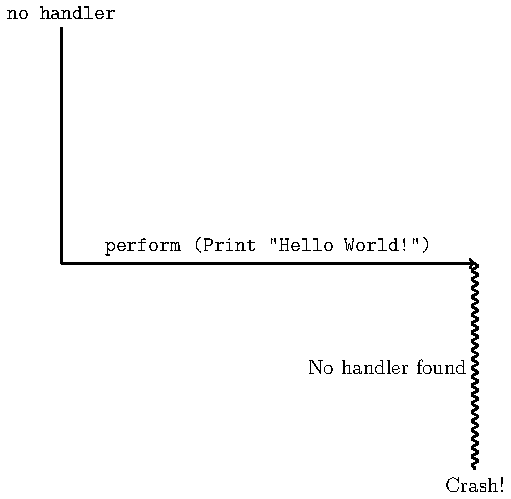
\includegraphics[width=.625\linewidth]{../figures/exception_control_flow.pdf}

  \caption{Crash without a handler.}
  \label{fig:exception}
\end{subfigure}
\begin{subfigure}{.5\textwidth}
  \centering
  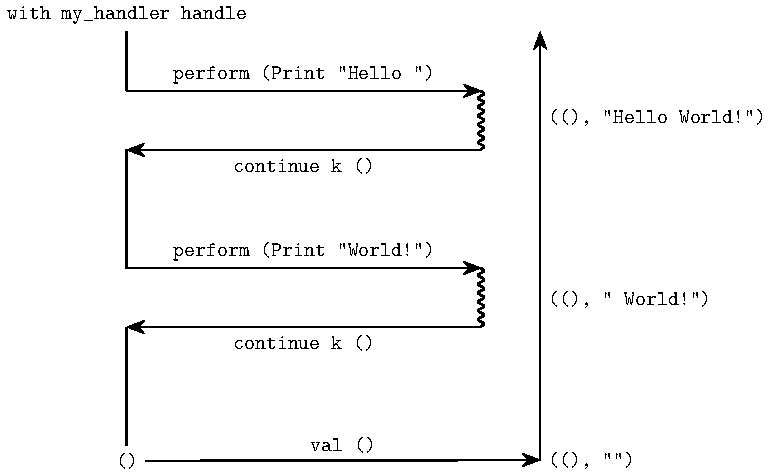
\includegraphics[width=\linewidth]{../figures/handler_hello_world.pdf}

  \caption{Effects and resumed continuations.}
  \label{fig:exception}
\end{subfigure}
\caption{The tutorial illustrated}
\end{figure}

\section{Continuations and control operators}
\label{section-continuations}

Although continuations came up briefly in the previous section I did not
explain what they are in detail. This section is devoted to this because
continuations are playing a crucial rôle in Eff and in what follows in this
dissertation.

\subsection{CPS in Scheme}
\lstset{language=scheme}

Continuations can represent an arbitrary program point in the execution of a
program and thus one can say that continuations are always there, whenever a
program executes. But where? A programming style called \emph{continuation
passing style} (CPS) is a style of programming where every function of $n$
arguments is rewritten to an extended version taking $n+1$ arguments, the last
of which is commonly named $k$ and represents a continuation.

Consider the Scheme code snippet in \autoref{cps-arithmetic} which uses this style to redefine the
built-in binary addition and multiplication functions of Scheme as ternary
functions \lstinline|+k| and \lstinline|*k| with an extra argument \verb|k|.
Also note how the expression \lstinline|(1 + 2)*(3 + 4)| is written in this
style.

\mylisting{scheme}
{$(1+2) * (3+4)$ in CPS}
{cps-arithmetic}
{../code_examples/cps_arithmetic.scheme}

We see that continuation passing style makes the order of the operations
explicit as well as it makes it obvious \emph{what} the continuation is.
However, writing code in this style is a bit troublesome and hence CPS is mostly
used as an intermediate representation of programs in compilers---not
something humans interact with.

\subsection{Scheme's call/cc}

Scheme is interesting from the point of view of continuations because it has the
\lstinline|call-with-current-continuation| built-in operation which is
conventionally referred to as \lstinline|call/cc|\footnote{A similarly obscure control operator is Peter Landin's J operator
which predates \lstinline{call/cc} by almost a decade. It was discovered shortly
after Peter Landin described SECD machines for the first time.}.
\emph{The call/cc operator takes a single argument. This argument is a \emph{function}
which itself takes a \emph{continuation} as an argument.}

If one wished to use continuations as first-class values in a Scheme program
one would not have to write everything in CPS like in \autoref{cps-arithmetic}. A similar piece of
code can be written with call/cc:

\mylisting{scheme}
{Continuations with \lstinline{call/cc} are not delimited}
{callcc-not-delim}
{../code_examples/callcc_not_delim.scheme}

Looking at line 7 we see that the continuation here returns to the toplevel.
Call/cc captures the continuation of the \emph{whole} program and
\emph{does not} return to the program point the continuation was called from.
This is different from how this is done in Eff.

\subsection{Delimited continuations}

Eff uses delimited continuations. These continuations \emph{do not} represent
the rest of the whole program. They represent the continuation
\emph{of the computation enclosed by a with-handle block}.

\mylisting{efflang}
{[Delimited continuations in Eff are functions]In Eff continuations behave like functions}
{continuations-as-functions}
{../code_examples/continuations_as_functions.eff}

In \autoref{continuations-as-functions} \lstinline{x} takes the value \lstinline{((), "Hello World")}
rather than \lstinline{42} which one would expect with Scheme's
\lstinline|call/cc|. The fact that continuations are delimited also makes it
possible to return to the program point a continuation was called from. This
also allows us to resume continuations in Eff more than once if necessary.
Hence, in Eff we can think about delimited continuations simply as functions.

\section{Eff formally}

\subsection{Syntax}

In the abstract syntax of Eff there is a distinction between pure expressions
and computations which are possibly effectful\footnote{The reader familiar with monads might discover some similarities
between \emph{val} and \emph{return} as well as similarities between monadic
type constructors and computations.}.

\begin{myfigure}[.9]{htb}{Abstract syntax of Eff}{fig:eff-syntax}
Effect declarations
$$ \effEffect E : A \tto B $$
%
Expressions
$$ e ::= x \mid
  \effTrue \mid
  \effFalse \mid
  () \mid
  (e_1, e_2) \mid
  \effLeft e \mid
  \effRight e \mid
  \effFun x \mapsto c \mid
  h $$
%
Handlers
$$ h ::= \effHandler \effVal x \mapsto c_v\ \overline{\parallel \ \effEffect E_i\ x\ k \to c_{\effOp_i} } \dmid \effFinally x \mapsto c_f $$
%
Computations
\begin{align*}
  c ::= \ &\effVal e \mid \effAbsurd e \mid
    \effLet x = c_1 \effIn c_2 \mid
    \effLet \effRec f\ x = c_1 \effIn c_2 \mid e_1\ e_2 \mid \\
    & \effIf e \effThen c_1 \effElse c_2 \mid
    \effMatch e\ \effWith \effLeft x \mapsto c_l \dmid \effRight y \mapsto c_r \mid\\
    & \effMatch e\ \effWith (f, s) \mapsto c \mid \effPerform (E\ e) \mid
    \effWith e \effHandle c
\end{align*}
\end{myfigure}

Most terms should be familiar to the reader by now. However, there are some
differences between the concrete and the abstract syntax of Eff. Notably, the
use of the \emph{val} keyword is omitted many times from the concrete syntax
because for programmers it might be tiresome if they have to keep track whether
they are writing an expression or a computation at the moment. The
\emph{continue} keyword is missing from the abstract syntax too. However, our
ability to resume computations did not vanish. As we saw in the previous section,
delimited continuations are just simply functions reifying a continuation. Hence
we can handle resumptions as function application. Anyhow, to ease the
understanding of the semantic rules I use the notation $(y.c)$ for delimited
continuations which resume the computation $c$ after receiving $y$.

\subsection{Semantics}

This section presents the small step operational semantics of Eff. The spotlight
is on possibly effectful computations and on their reduction rules given by the
relation $\leadsto$. I focus on the Eff specific transition steps here (see
\autoref{fig:mini-semantics}). The other transition rules are standard and can
be found in Appendix \ref{app:theory}.

\begin{myfigure}[1]{htb}
  {Eff-specific rules of the small step operational semantics}
  {fig:mini-semantics}
  $$
  \begin{prooftree}
    \hypo{c_1 \leadsto c_1'}
    \infer1[(\textsc{Let-Step})]{\effLet x = c_1 \effIn c_2 \leadsto \effLet x = c_1' \effIn c_2}
  \end{prooftree}
  $$

  $$
  \begin{prooftree}
    \hypo{}
    \infer1[(\textsc{Let-Val})]{\effLet x = (\effVal e) \effIn c \leadsto c[e/x]}
  \end{prooftree}
  $$
  
  $$
  \begin{prooftree}
    \hypo{}
    \infer1[(\textsc{Let-Effect})]{\effLet x = E(e, y.c_1) \effIn c_2 \leadsto E(e, y.\effLet x = c_1 \effIn c_2)}
  \end{prooftree}
  $$

  $$
    \begin{prooftree}
      \hypo{\kappa \text{ is current delimited continuation}}
      \infer1[(\textsc{Perform})]{\effPerform (E\ e) \leadsto E(e, \kappa)}
    \end{prooftree}
    $$

    $$
    \begin{prooftree}
      \hypo{c \leadsto c'}
      \infer1[(\textsc{Handle-Step})]{\effWith e \effHandle c \leadsto \effWith e \effHandle c'}
    \end{prooftree}
    $$
    
    $$
    \begin{prooftree}
      \hypo{h \stackrel{\text{def}}{=} (\effHandler \effVal x \mapsto c_v \dmid \dots)}
      \infer1[(\textsc{Handle-Val})]{\effWith h \effHandle (\effVal e) \leadsto c_v[e/x]}
    \end{prooftree}
    $$
    
    $$
    \begin{prooftree}
      \hypo{h \stackrel{\text{def}}{=} (\effHandler \dots \overline{\dmid \effEffect E_i\ x\ k \mapsto c_i} \dmid \dots)}
      \hypo{\exists i. E_i = E}
      \infer2[(\textsc{Handle-Eff-Match})]{\effWith h \effHandle E(e, y.c) \leadsto c_i[e/x, (y.c)/k]}
    \end{prooftree}
    $$
    
    $$
    \begin{prooftree}
      \hypo{h \stackrel{\text{def}}{=} (\effHandler \dots \overline{\dmid \effEffect E_i\ x\ k \mapsto c_i} \dmid \dots)}
      \hypo{\forall i. E_i \neq E}
      \infer2[(\textsc{Handle-Eff-Rise})]{\effWith h \effHandle E(e, y.c) \leadsto E( e, y. \effWith h \effHandle c)}
    \end{prooftree}
    $$
\end{myfigure}

The explanation of these rules is given by \autoref{tab:semantics-rule-explanation}
so that the reader can quickly jump between the comments there and the rules on
\autoref{fig:mini-semantics}.

\begin{table}
  \small
  \centering
  {\renewcommand{\arraystretch}{1.3}
  \rowcolors{2}{gray!17}{white}
  \begin{tabularx}{\textwidth}{lX}
  \toprule
  Rule & Comment \\
  \midrule
  \textsc{Let-Val} & 
    If a computation \emph{returns} an expression $e$, it is bound to the
    identifier $x$ in the computation $c$. \\

  \textsc{Let-Effect} & 
    A computation $c$ can also reduce to a \emph{performed effect} $E(e, y.c_1)$,
    where $e$ is the argument of the effect constructor and $(y.c_1)$ is a
    delimited continuation representing the program point $c$'s execution was
    stopped at. This delimited continuation can be used later to resume $c$. \\

  \textsc{Perform} &
    Whenever we perform an effect, a so-called \emph{effect packet} (similar to
    \emph{exception packets} in SML, see \cite{paulson1996ml}) $E(e, \kappa)$
    is created. Here, $e$ is the argument to the effect and $\kappa$ is the
    captured delimited continuation which is determined by the with-handle
    blocks surrounding this computation. Note, that because it is not guaranteed
    that there are such with-handle blocks around a $\effPerform$call, creating
    such an effect package might not always be possible. \\

  \textsc{Handle-Val} & 
    If a computation in a with-handle block with handler $h$ reduces to
    $\effVal e$, then the \emph{value case} of $h$ (i.e., $\effVal x \mapsto c_v$)
    is invoked by substituting $e$ for $x$ in $c_v$. \\

  \textsc{Handle-Eff-Match} &
    This rule tells us what happens when there is a \emph{matching effect case}
    in the current handler. The argument of the effect is bound to $x$ and the
    delimited continuation $(y.c)$ is bound to $k$. \\

  \textsc{Handle-Eff-Rise} &
    This rule tells us what happens when the next handler \emph{cannot} handle
    the effect which was performed. In this case the effect packet is modified
    which is quite important. The \emph{body} of the delimited continuation is
    surrounded by the current non-matching with-handle block. This achieves the
    effect that when the continuation is resumed we also \emph{restore all the
    handlers we escaped} when we were ``searching'' for a matching handler.
    This is a property of the semantics which we will have to be very careful
    about when implementing the CEK interpreter and the SHADE VM in the next
    chapter.\\

  \bottomrule
  \end{tabularx}
  \caption[Small step operational semantics of Eff]{Explanation of the Eff specific rules of the small step semantics}
  \label{tab:semantics-rule-explanation}
  }
\end{table}

\subsection{Types}

The types of Eff are as follows:
  $$A ::= 
    b \mid
    \mathtt{bool} \mid
    \mathtt{unit} \mid
    \mathtt{empty} \mid
    A * B \mid
    A + B \mid
    A \to B \mid
    A \Rightarrow B$$
  $$ E_i ::= A_i \tto B_i $$
%
where $b$ stands for built-in types (e.g., my implementation includes built-in
types such as ints, reals and strings) which are not particularly interesting
here. In the following section we assume the existence of a set $\Sigma_E$
containing all \emph{effect signatures} of the form $E_i : A_i \tto B_i$.

\subsubsection{Type checking}

Again, I omit standard typing rules and focus on the Eff specific ones. For the
sake of completeness Appendix \autoref{app:theory} contains the other rules.
There are two separate typing relations denoted $\vdash_e$ and $\vdash_c$ for
expressions and computations respectively. Type environments are denoted
$\Gamma$ and are maps from variable names to types.

\begin{myfigure}[1]{htb}
{Type checking for Eff-specific expressions and computations}
{fig:type-checking-expressions}

$$
    \begin{prooftree}
      \hypo{\Gamma \vdash_e e : A}
      \infer1[(\textsc{T-Val})]{\Gamma \vdash_c \effVal e : A}
    \end{prooftree}
    \quad
    \begin{prooftree}
      \hypo{\Gamma \vdash_e e : A \handlerType B}
      \hypo{\Gamma \vdash_c c : A}
      \infer2[(\textsc{T-WHandle})]{\effWith e \effHandle c : B}
    \end{prooftree}
  $$

  $$
    \begin{prooftree}
      \hypo{E : A \tto B \in \Sigma_E}
      \hypo{\Gamma \vdash_e e : A}
      \infer2[(\textsc{T-Perform})]{\effPerform (E\ e) : B}
    \end{prooftree}
    \quad
    \begin{prooftree}
      \hypo{\Gamma \vdash_e e : \emptyType}
      \infer1[(\textsc{T-Absurd})]{\Gamma \vdash_c \effAbsurd e : A}
    \end{prooftree}
  $$

  \begin{align*}
    {\begin{prooftree}
      \hypo{x : A, \Gamma \vdash_c c_v : C}
      \hypo{\forall i.\ e_i : A_i, k_i : B_i, \Gamma \vdash_c c_i : C}
      \hypo{x : C, \Gamma \vdash_c c_f : D}
      \infer3[(\textsc{T-Handler})]{\Gamma \vdash_e h : A \handlerType D}
    \end{prooftree}}\\
    \text{ where }
    h \defEq (
      \effHandler
        \effVal x \mapsto c_v
        \overline{\dmid \effEffect E_i\ e_i\ k_i \mapsto c_i} \dmid
        \effFinally x \mapsto c_f)
    \text{ and } \\ \forall i.\ E_i : A_i \tto B_i \in \Sigma_E
  \end{align*}
\end{myfigure}
%
Again, explanation of these rules is given in
\autoref{tab:typing-rule-explanation} in a similar way to how it was done for
the semantics.

\begin{table}
  \small
  \centering
  {\renewcommand{\arraystretch}{1.3}
  \rowcolors{3}{gray!17}{white}
  \begin{tabularx}{\textwidth}{lX}
  \toprule
  Rule & Comment \\
  \midrule
  \textsc{T-Val} &
    This rule is standard. The expression $e$ and the computation $\effVal e$ are given the same type.\\
  \textsc{T-Perform} &
    This rule is similar to function application for effects.\\
  \textsc{T-Handler} &
    The rule for typing handlers might be the scariest one. We are saying here that
    the type of the value- and effect cases must agree (this is type $C$ in the rule) and that
    the finally case which takes something of type $C$ and gives something of type $D$ transform a
    value of type $C$ into something of type $D$. The resulting handler type $A \handlerType D$ reflects
    this by saying that a computation of type $A$ will be turned into one of type $D$ by such a handler, when it
    is applied.\\
  \textsc{T-WHandle} &
    As applying handlers happens with with-handle blocks this rule is similar to
    the function application typing too. \\
  \bottomrule
  \end{tabularx}
  \caption[Eff typing]{Explanation of the Eff specific typing rules}
  \label{tab:typing-rule-explanation}
  }
\end{table}

\lstset{language=efflang}

The attentive reader might have wondered what $\effAbsurd$and the $\emptyType$
type are good for. In the tutorial we got away with a slight lie which we will
make amends for here. We said that in the absence of suitable handlers an effect
will behave like an exception (remember \autoref{first-example}). This is
not quite true when typing is introduced, as a computation like
%
\begin{center}
\begin{tabular}{c}
{\begin{lstlisting}[language=efflang, numbers=none, frame=none]
effect Error of string -->> unit;;
if true then (perform (Error "Lie detected")) else 1337
\end{lstlisting}}
\end{tabular}
\end{center}
%
won't be typeable with our rules (there is a type mismatch between $\unitType$
and $\mathtt{int}$), although in OCaml or SML one can write
%
\begin{center}
\begin{tabular}{c}
{\begin{lstlisting}[language=caml, numbers=none, frame=none]
exception Error of string;;
if true then (raise (Error "Lie detected!")) else 1337
\end{lstlisting}}
\end{tabular}
\end{center}
%
without any problems. We would like to use effects as exceptions---it would be
weird not to, as they are a generalisation of them. This is why we need
$\effAbsurd$and the $\emptyType$ type. We can now say
\\
\mylisting{efflang}
{Absurd and empty with exceptions}
{absurd-and-empty}
{../code_examples/absurd_empty.eff}
%
and this will type check if we use (\textsc{T-Absurd}). Note also that the only
way one can introduce the $\emptyType$ type is by declaring an effect that has
an $\emptyType$ output.

The distinction between pure expressions and effectful computations allows for
the use of an \emph{effect system} with these rules. For instance, if one were
to extend these rules with \emph{row-typing} one could keep track of what kind
of side effecting computations occur in different parts of the program. This can
aid reasoning about programs, help us to discover more optimisations by using
type and effect information and to ensure that programs have certain safety
properties. These are nice to have features and are outside of the scope of this
dissertation.

\section{Abstract machines by example}

A purist would look at rule \textsc{(Perform)} in \autoref{fig:mini-semantics}
and would think that the phrasing of the hypothesis is troublesome. I actually
think that this ambiguity reflects well the challenge in this project. Consider
for instance implementing an interpreter on the source terms of a language X.
One's first instinct is that this is a trivial task: all we need to do is to
write a recursive evaluator function, something of this sort:

\mylisting{caml}
{[A naïve recursive evaluator] A naïve recursive evaluator function might look like this}
{naive-implementation}
{../code_examples/naive_implementation.ml}

Indeed, this works for most programming languages (ones that do not have control
operators like continuations) and this was my first attempt when writing a
\nth{0} prototype in the very early stages of the project. I started to struggle
when I reached the point I had to deal with continuations, as I needed the
ability to access $\kappa$ any time in the evaluation of a program. But
evaluators of this kind do not lend themselves easily to such maneuvers.

Hence this section is concerned with two types of abstract machines which are
capable of doing what is described above. I will illustrate how they do this on
a toy language and by the end of this section we will be able to discover a
correspondence between the \emph{runtime representation} of continuations in
these machines and the CPS Scheme example from \Cref{section-continuations}.

These two machines are CEK and SECD machines. They both interpret source terms
directly and this makes it easy to implement them (a CEK implementation of Eff
is discussed in the Implementation chaper).

Consider the following Toy Language (TL), which is the untyped lambda calculus
with natural numbers as values and with built-in operations like addition and
multiplication:
$$ t ::= x \mid n \mid \lambda x. t \mid t_0\ t_1 \mid t_0 + t_1 \mid t_0 * t_1.$$
Our dummy example from \Cref{section-continuations} in TL will be:
$$ \mathtt{plus} = \lambda x. \lambda y.\ x + y $$
$$ \mathtt{times} = \lambda x. \lambda y.\ x * y $$
$$ \mathtt{times}\ (\mathtt{plus}\ 1\ 2)\ (\mathtt{plus}\ 3\ 4).$$
What follows is a brief description of CEK and SECD machines for TL illustrated
on this example.

\subsection{CEK machines}

As the name suggests, the state of CEK machines consists of three components:
\emph{control} (C), \emph{environment} (E) and \emph{kontinuation} (K). Control
is simply the program to be evaluated in its abstract syntax tree form.
Environment is a mapping from variable names to values (in our case, the natural
numbers) and kontinuation is a \emph{stack of closures} representing the rest
of the program to be interpreted at any given time. Hence a configuration of the
machine is characterised by a three-tuple $\cek{C, E, K}$.

\begin{myfigure}[.9]{t}
{CEK machine transition rules for TL}
{fig:cek-tl}
\small
Initialisation:
$$ t \to \cek{t, \{\}, nil} $$
%
Transition rules:
$$ \cek{x, E, (y.t, E') :: K} \to \cek{E(x), E, K} $$
$$ \cek{v, E, (y.t, E') :: K} \to \cek{t, E'[y \mapsto v], K} \quad (*)$$
$$ \cek{(\lambda y. t_1)\ t_2, E, K} \to \cek{t_2, E, (y.t_1, E) :: K} $$
$$ \cek{t_1 + t_2, E, K} \to \cek{\mathtt{add}(t_1, t_2), E, K} $$
$$ \cek{t_1 * t_2, E, K} \to \cek{\mathtt{mult}(t_1, t_2), E, K} $$
$$ \cek{\mathtt{op}(t_1, t_2), E, K} \to \cek{t_1, E, (y.\mathtt{CONT1}(y, \mathtt{op}, t_2), E) :: K} \text{ for a \emph{fresh} $y$} $$
$$ \cek{\mathtt{CONT1}(x, \mathtt{op}, t_2), E, K} \to \cek{t_2, E, (y.\mathtt{CONT2}(x, \mathtt{op}, y), E) :: K} \text{ for a \emph{fresh} $y$} $$
$$ \cek{\mathtt{CONT2}(x, \mathtt{op}, y), E, K} \to \cek{v, E, K} \text{ where } v = \mathtt{op}(x, y) $$
%
Termination:
$$ \cek{x, E, nil} \to E(x) $$
$$ \cek{v, E, nil} \to v $$
\end{myfigure}

We see at $(*)$ in \autoref{fig:cek-tl} that whenever we reduce a term to a value $v$, a continuation
$(y.t)$ is popped off the K stack, $v$ is bound to the variable $y$ in $E'$
(this is the environment we need to restore to be able to interpret $t$ in the
same context we stopped evaluating its parent expression) and then $t$ is
resumed. We need to use \emph{two} types of continuations for TL as it has
\emph{binary} operators $+$ and $*$. The name \texttt{CONT1} suggests that one
of the operands is reduced to a value and one remains to be reduced before the
actual operation can be performed. \texttt{CONT2} is used to represent the state
when both of the operands are values and the operation \texttt{op} can be
performed (be that the built-in \texttt{add} or \texttt{mult}).

We see that a $\effPerform$ operation would be easier to implement in this
representation than in the naïve way. Furthermore, we should notice that a CPS
transformation is done on the terms ``on the fly'' during the evaluation and we
benefit from this because this avoids us (programmers) having to make the
continuations explicit in our programs by writing them in CPS.

\subsection{The SECD machine}

SECD machines originate from Landin's famous
\emph{The mechanical evaluation of expressions} \cite{landin-secd}. Their state
is characterised by four components, namely: a \emph{stack} (S),
an \emph{environment} (E), a \emph{control} (C) and a \emph{dump} (D). The first
three components are standard. Here the rôle of dump is similar to the rôle of
$K$ in the CEK machine. It is a list of three tuples, each three tuple consisting
of the other three components (i.e., it has the form $(S, E, C)$). The dump
embodies a list of saved execution contexts we can return to if we wish.

\begin{myfigure}[.8]{htb}
{SECD machine transition rules for TL}
{fig:secd-transitions}
\small
Initialisation:
$$ t \to \secd{nil, \{\}, [t], nil} $$
%
Transition rules:
$$ \secd{S, E, x :: C, D} \to \secd{E(x) :: S, E, C, D} $$
$$ \secd{v :: S, E, nil, (S', E', C') :: D} \to \secd{v :: S', E', C', D} $$
$$ \secd{S, E, (t_1\ \mathtt{op}\ t_2 :: C, D} \to \secd{S, E, t_1 :: t_2 :: \mathtt{op} :: C, D} $$
$$ \secd{S, E, (t_1\ t_2) :: C, D} \to \secd{S, E, t_2 :: t_1 :: \mathtt{ap} :: C, D} $$
$$ \secd{(y, E', t) :: v :: S, E, \mathtt{ap} :: C, D} \to \secd{nil, E'[y \mapsto v], [t], (S, E, C) :: D} $$
$$ \secd{v_2 :: v_1 :: S, E, \mathtt{op} :: C, D} \to \secd{v :: S, E, C, D} \text{ for } v = \mathtt{op}(v_1, v_2) $$
%
Termination:
$$ \secd{v :: S, E, nil, nil} \to v $$
\end{myfigure}

\begin{figure}[htb]
  \begin{subfigure}{.5\textwidth}
    \subcaptionbox{
        \emph{Naïve approach.} Imagine that a $\effPerform$ operation is
        issued at position 2 in the tree. As the naïve approach only keeps track
        of the continuations implicitly we cannot represent the red arrow easily.
    }
    [8cm][c]
    {\resizebox{\textwidth}{!}{\subimport{../figures/}{naive.tex}}}
    \label{fig:continuation-naive}
  \end{subfigure}
  %
  \begin{subfigure}{.5\textwidth}
    \subcaptionbox{
        \emph{SECD machine.} The stack of the SECD machine is a
        representation of the red arrow from (\subref{fig:continuation-naive}).
        However, SECD does not need to pass values around between closures like
        (\subref{fig:continuation-cek}) does.
    }
    [8cm][c]
    {\resizebox{\textwidth}{!}{\subimport{../figures/}{secd.tex}}}
    \label{fig:continuation-secd}
  \end{subfigure}
  %
  \begin{subfigure}{\textwidth}
    \centering
    \resizebox{\textwidth}{!}{
      \subimport{../figures/}{cek.tex}
    }
    \caption{\emph{CEK machine.} The $K$ component of the CEK machine represents
    continuations with closures the same way our continuations were nested in each other in the
    Scheme example.}
    \label{fig:continuation-cek}
  \end{subfigure}
  %
  \caption{Where is the continuation?}
  \label{fig:naive-cek-secd}
\end{figure}

We see that although this machine works on abstract syntax trees, it is still a
bit lower level than the CEK machine in that it makes a stack explicit and the
way it processes (disassembles) the tree is very similar to compiling. In
control, we end up with a list of smaller trees and SECD instructions.
With just another step we can turn this into a stack machine and this is what I will
do in the Implementation chapter.

\paragraph{Importance}
\autoref{fig:naive-cek-secd} sums up why this section is important. It is an
illustration of how different evaluators represent continuations. Note that the
representation of a continuation in \autoref{fig:naive-cek-secd}\subref{fig:continuation-secd} looks
very similar to an instruction stream. It is as if CEK did a CPS translation on
the fly while SECD did both a CPS and a ``sort of compilation'' while
interpreting a program---this is a precious insight to possess when our task is to
compile a language like Eff!

\section{Software engineering}

\subsection{Licensing}

It is important to mention that the project fulfills licensing criteria. The
dependencies of this project are listed below with their licenses:
\begin{itemize}
\item The OCaml toplevel, version 4.06.0, GNU LGPL version 2.1
\item \emph{menhir} parser generator, version 20190924, GNU GPL version 2
\item \emph{Alcotest}, version 0.8.5, ISC license
\item \emph{OCaml Package Manager}, version 2.0.4, GNU LGPL version 2.1
\item \emph{Core} standard library by Jane Street, v0.11.3, MIT license
\end{itemize}
To the best of my knowledge these licenses allow the way I am using the software
mentioned above.

\subsection{Starting point}

The starting point of my project did not change since the writing of the
project proposal (see Appendix \ref{project-proposal}):
\begin{itemize}
  \item I read briefly about Eff and algebraic effect handlers before starting
  my project.
  \item I used SML and OCaml before to implement simple interpreters for toy
  programming languages and to experiment with functional programming. This is
  my first big project where I use functional programming.
  \item I also had a look at the OCaml ecosystem to check if it has a stable
  build system, if testing frameworks are available and whether lexer and parser
  generators exist.
\end{itemize}

\subsection{Development methodology}

I chose \emph{test-driven development} (TDD) \cite{beck2003test} as my project's
software development methodology. The essence of TDD is that programmers work in
quick iterative cycles whereby they write failing tests first and then implement
the next feature that makes the failing test cases pass. Always having an
\emph{automated} test suite at hand avoids trial and error testing which would
be both error prone and time consuming. The reasons for choosing this
methodology was three-fold.

Firstly, the nature of my project is such that the correctness of any code
written is very well-defined as I can take the semantics of Eff as a baseline
and given a piece of code it is always possible to tell whether it is
interpreted correctly or not. This makes it possible to write tests upfront.

Second, the structure of my project imposed an order on the parts to be
delivered. This is because every module of my project (apart from the front end)
depends on a previous one and hence on its correctness. As TDD is also known as 
``a way of managing fear during programming'' it came handy that I could write
code with confidence knowing that the code I have written before is tested.
Other advantages were the ability to notice quickly if a code change broke some
already implemented feature and the ability to refactor code with confidence
(which I had to do frequently---from summer internships I knew that my coding
style is such that this will be unavoidable if I want to work with a
maintainable codebase).

Third, my success criterion was a correct working implementation of a compiler,
so tests were crucial to demonstrate that success criteria were fulfilled.

\section{Summary}
This section summed up the theoretical background which was needed to complete
this project. It also shows the preparation I undertook in the software
engineering aspects.

\begin{itemize}
\item Eff was introduced in a brief tutorial.
\item It was explained how continuations represent arbitrary program points
        in the execution of a program. Therefore they can be used to implement
        advanced control flow.
\item \emph{Core Eff} was formally introduced.

\item Two abstract machines (CEK and SECD machines) were introduced.
    These can implement the structured \emph{non-local flow of control}
    continuations make possible. The key challenge these machines solve is that
    they can \emph{save and restore} execution contexts in an appropriate way
    whenever non-local control flow has to occur.

    A CEK machine does this by keeping a stack of continuations (K), while the
    SECD machine does this by using a so-called dump (D). The importance of
    these machines will become clearer in the Implementation section where I
    describe the SHADE virtual machine for Eff which has similarities with both
    of these abstract machines.

\item I stated my starting point and discussed the development methodology
    used to write the code and the testing strategy to assess its correctness.
\end{itemize}

\ifstandalone
\bibliography{../bibliography}{}
\bibliographystyle{plain}
\fi

\end{document}
